\documentclass[10pt]{article}\usepackage[]{graphicx}\usepackage[]{color}
%% maxwidth is the original width if it is less than linewidth
%% otherwise use linewidth (to make sure the graphics do not exceed the margin)
\makeatletter
\def\maxwidth{ %
  \ifdim\Gin@nat@width>\linewidth
    \linewidth
  \else
    \Gin@nat@width
  \fi
}
\makeatother

\definecolor{fgcolor}{rgb}{0.345, 0.345, 0.345}
\newcommand{\hlnum}[1]{\textcolor[rgb]{0.686,0.059,0.569}{#1}}%
\newcommand{\hlstr}[1]{\textcolor[rgb]{0.192,0.494,0.8}{#1}}%
\newcommand{\hlcom}[1]{\textcolor[rgb]{0.678,0.584,0.686}{\textit{#1}}}%
\newcommand{\hlopt}[1]{\textcolor[rgb]{0,0,0}{#1}}%
\newcommand{\hlstd}[1]{\textcolor[rgb]{0.345,0.345,0.345}{#1}}%
\newcommand{\hlkwa}[1]{\textcolor[rgb]{0.161,0.373,0.58}{\textbf{#1}}}%
\newcommand{\hlkwb}[1]{\textcolor[rgb]{0.69,0.353,0.396}{#1}}%
\newcommand{\hlkwc}[1]{\textcolor[rgb]{0.333,0.667,0.333}{#1}}%
\newcommand{\hlkwd}[1]{\textcolor[rgb]{0.737,0.353,0.396}{\textbf{#1}}}%
\let\hlipl\hlkwb

\usepackage{framed}
\makeatletter
\newenvironment{kframe}{%
 \def\at@end@of@kframe{}%
 \ifinner\ifhmode%
  \def\at@end@of@kframe{\end{minipage}}%
  \begin{minipage}{\columnwidth}%
 \fi\fi%
 \def\FrameCommand##1{\hskip\@totalleftmargin \hskip-\fboxsep
 \colorbox{shadecolor}{##1}\hskip-\fboxsep
     % There is no \\@totalrightmargin, so:
     \hskip-\linewidth \hskip-\@totalleftmargin \hskip\columnwidth}%
 \MakeFramed {\advance\hsize-\width
   \@totalleftmargin\z@ \linewidth\hsize
   \@setminipage}}%
 {\par\unskip\endMakeFramed%
 \at@end@of@kframe}
\makeatother

\definecolor{shadecolor}{rgb}{.97, .97, .97}
\definecolor{messagecolor}{rgb}{0, 0, 0}
\definecolor{warningcolor}{rgb}{1, 0, 1}
\definecolor{errorcolor}{rgb}{1, 0, 0}
\newenvironment{knitrout}{}{} % an empty environment to be redefined in TeX

\usepackage{alltt}

\usepackage{amsmath,amssymb,amsthm}
\usepackage{fancyhdr,url,hyperref}
\usepackage{graphicx,xspace}
\usepackage{subfigure}
\usepackage{tikz}
\usetikzlibrary{arrows,decorations.pathmorphing,backgrounds,positioning,fit,through}

\oddsidemargin 0in  %0.5in
\topmargin     0in
\leftmargin    0in
\rightmargin   0in
\textheight    9in
\textwidth     6in %6in
%\headheight    0in
%\headsep       0in
%\footskip      0.5in

\newtheorem{thm}{Theorem}
\newtheorem{cor}[thm]{Corollary}
\newtheorem{obs}{Observation}
\newtheorem{lemma}{Lemma}
\newtheorem{claim}{Claim}
\newtheorem{definition}{Definition}
\newtheorem{question}{Question}
\newtheorem{answer}{Answer}
\newtheorem{problem}{Problem}
\newtheorem{solution}{Solution}
\newtheorem{conjecture}{Conjecture}

\pagestyle{fancy}

\lhead{\textsc{Prof. McNamara}}
\chead{\textsc{SDS/MTH 220: Lecture notes}}
\lfoot{}
\cfoot{}
%\cfoot{\thepage}
\rfoot{}
\renewcommand{\headrulewidth}{0.2pt}
\renewcommand{\footrulewidth}{0.0pt}

\newcommand{\ans}{\vspace{0.25in}}
\newcommand{\R}{{\sf R}\xspace}
\newcommand{\cmd}[1]{\texttt{#1}}

\rhead{\textsc{October 18, 2017}}
\IfFileExists{upquote.sty}{\usepackage{upquote}}{}
\begin{document}

\paragraph{Agenda}
\begin{enumerate}
  \itemsep0em
  \item Confidence intervals
  \item Central limit theorem
  \item Sampling Distributions from Multimodal Populations
\end{enumerate}


\paragraph{Reminder}

Confidence intervals for test statistics that are normally distributed are of the form:
$$
  \text{point estimate} \pm z_{\alpha/2}^* \cdot SE
$$
Computing the point estimate is usually easy. Once you've chosen a confidence level, finding $z_{\alpha/2}^*$ is trivial (use \cmd{qnorm()} or the table in the back of the book). The difficult part is usually computing the $SE$, since that depends on the sampling distribution of the test statistic!

\paragraph{Warmup}

  \begin{enumerate}
    \itemsep0in
    % MMC, 7e, 6.21
    \item A recent study estimated the mean U.S. per capita consumption of sugar-sweetened beverages among adults 20 to 44 years of age to be 289 kcal/day with a standard error of 7 kcal/day.
    \begin{enumerate}
      \itemsep0.3in
      \item The 68-95-99.7 rule says that the probability is about 0.95 that $\bar{x}$ is within $y$ kcal/day of the population mean $\mu$. What is $y$? 
      \item About 99\% of all samples will capture the true mean of kcals consumed per day in the interval $\bar{x}$ plus or minus $7$ kcal/day times what? Draw a labeled picture and indicate where the missing quantity is. Estimate it. What does the computer need to known in order to compute it? 



      \vspace{0.2in}
    \end{enumerate}
    % MMC, 7e, 6.13
    \item Suppose 400 randomly selected alumni of the University of Okoboji were asked to rate the university's counseling services on a 1 to 10 scale. The sample mean was found to be 8.6. Assume that the standard error was computed to be 0.4. 
    \begin{enumerate}
      \itemsep0.4in
      \item A researcher computes the 99\% confidence interval for the average satisfaction score as $8.6 \pm 1.96 \cdot 0.4$. What is her mistake? 
      \item After correcting her mistake in part (a), she states: ``I am 95\% confident that the sample mean falls between 7.82 and 9.38." What is wrong with this statement?
      \item She quickly realizes her mistake in part (b) and instead states: ``The probability the true mean is between 7.82 and 9.38 is 0.95." What misinterpretation is she making now? 
      \item Finally in her defense for using the Normal distribution to determine the confidence interval she says ``Because the sample size is quite large, the population of alumni ratings  will be approximately Normal." Explain to Ima her misunderstanding and correct this statement.
    \end{enumerate}
  
      \vspace{0.2in}
    % MMC, 7e, 6.89
    \item Explain whether a test of signficance can answer each of the following questions.
    \begin{enumerate}
      \item Is the sample or experiment properly designed?
      \item Is the observed effect compatible with the null hypothesis?
      \item Is the observed effect important?
    \end{enumerate}
    
      % MMC, 7e, 6.92
    \item Justify whether or not you agree with each of the following statements.
    \begin{enumerate}
      \item If the p-value is larger than 0.05, the null hypothesis is true.
      \item Practical significance is not the same as statistical significance.
      \item We can perform a statistical analysis using any set of data.
      \item If you find an interesting pattern in a set of data, it is appropriate to then use a significance test to determine its significance.
    \end{enumerate}
  
  \end{enumerate}
  
\paragraph{Central limit theorem}

See \url{http://45.55.32.181/shiny/SamplingDist/}

\begin{enumerate}
\itemsep1in
\item What happens to the sampling distribution as the size of samples increases?
\item What happens to the sampling distribution as the number of samples increases?
\end{enumerate}
\vspace{1in}
\paragraph{Sampling Distributions from Multimodal Populations}

Consider the following multimodal probability distribution.

\begin{knitrout}\footnotesize
\definecolor{shadecolor}{rgb}{0.969, 0.969, 0.969}\color{fgcolor}\begin{kframe}
\begin{alltt}
\hlkwd{require}\hlstd{(mosaic)}
\hlstd{n} \hlkwb{<-} \hlnum{1000}
\hlstd{ds} \hlkwb{<-} \hlkwd{data.frame}\hlstd{(}\hlkwc{a} \hlstd{=} \hlkwd{rnorm}\hlstd{(n,} \hlkwc{mean} \hlstd{=} \hlnum{53}\hlstd{),} \hlkwc{b} \hlstd{=} \hlkwd{rnorm}\hlstd{(n,} \hlkwc{mean} \hlstd{=} \hlnum{57}\hlstd{,} \hlkwc{sd} \hlstd{=} \hlnum{0.8}\hlstd{),}
                 \hlkwc{c} \hlstd{=} \hlkwd{rnorm}\hlstd{(n,} \hlkwc{mean} \hlstd{=} \hlnum{64}\hlstd{),} \hlkwc{d} \hlstd{=} \hlkwd{rnorm}\hlstd{(n,} \hlkwc{mean} \hlstd{=} \hlnum{68}\hlstd{,} \hlkwc{sd} \hlstd{=} \hlnum{0.8}\hlstd{),} \hlkwc{p} \hlstd{=} \hlkwd{runif}\hlstd{(n))} \hlopt
  \hlkwd{mutate}\hlstd{(}\hlkwc{x} \hlstd{=} \hlkwd{ifelse}\hlstd{(p} \hlopt{<} \hlnum{0.25}\hlstd{, a,} \hlkwd{ifelse}\hlstd{(p} \hlopt{<} \hlnum{0.4}\hlstd{, b,} \hlkwd{ifelse}\hlstd{(p} \hlopt{<} \hlnum{0.65}\hlstd{, c, d))))}
\hlstd{pop_plot} \hlkwb{<-} \hlkwd{qplot}\hlstd{(}\hlkwc{data} \hlstd{= ds,} \hlkwc{x} \hlstd{= x,} \hlkwc{geom} \hlstd{=} \hlstr{"density"}\hlstd{,} \hlkwc{adjust} \hlstd{=} \hlnum{0.5}\hlstd{)} \hlopt{+}
  \hlkwd{geom_vline}\hlstd{(}\hlkwd{aes}\hlstd{(}\hlkwc{xintercept} \hlstd{=} \hlkwd{mean}\hlstd{(ds}\hlopt{$}\hlstd{x)),} \hlkwc{linetype} \hlstd{=} \hlnum{2}\hlstd{)}
\hlstd{pop_plot}
\end{alltt}
\end{kframe}
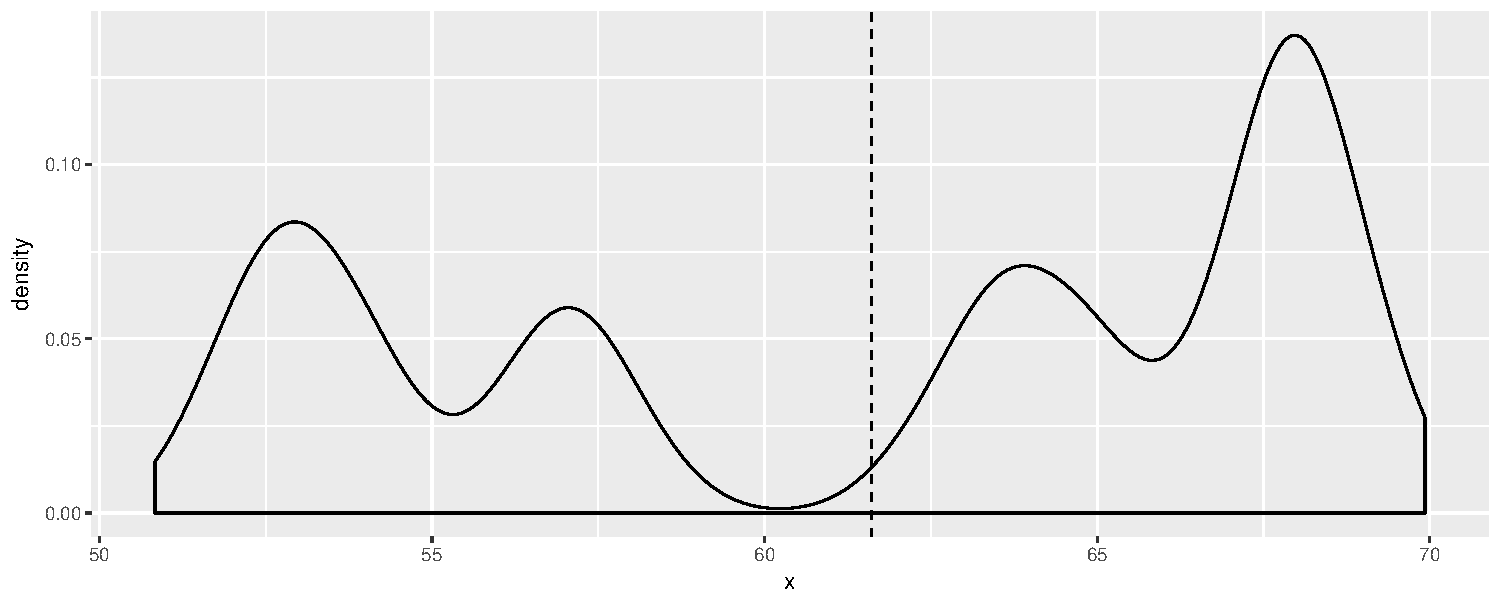
\includegraphics[width=\maxwidth]{figure/unnamed-chunk-2-1} 

\end{knitrout}

\begin{enumerate}
  \itemsep1in
    \item Sketch what you think the sampling distribution of the mean looks like for samples of size 1.
    \item Sketch what you think the sampling distribution of the mean looks like for samples of size 2.
    \item Sketch what you think the sampling distribution of the mean looks like for samples of size 10,000.
    \item Sketch what you think the sampling distribution of the mean looks like for samples of size 4.
  \end{enumerate}
  \vspace{1in}

\begin{knitrout}\footnotesize
\definecolor{shadecolor}{rgb}{0.969, 0.969, 0.969}\color{fgcolor}\begin{kframe}
\begin{alltt}
\hlstd{sim} \hlkwb{<-} \hlkwd{do}\hlstd{(}\hlnum{1000}\hlstd{)} \hlopt{*} \hlkwd{mean}\hlstd{(}\hlopt{~}\hlstd{x,} \hlkwc{data} \hlstd{=} \hlkwd{sample_n}\hlstd{(ds,} \hlnum{4}\hlstd{))}
\hlstd{pop_plot} \hlopt{+} \hlkwd{geom_density}\hlstd{(}\hlkwc{data} \hlstd{= sim,} \hlkwd{aes}\hlstd{(}\hlkwc{x} \hlstd{= mean),} \hlkwc{adjust} \hlstd{=} \hlnum{0.5}\hlstd{,} \hlkwc{color} \hlstd{=} \hlstr{"red"}\hlstd{)}
\end{alltt}
\end{kframe}
\end{knitrout}


\end{document}
